

CLIGen instantiates the NC abstraction in command-line interfaces.
Observations $x_t$ are terminal frames rendered from the underlying text buffer.
The conditioning stream $u_t$ carries a user prompt and optional metadata, and the video latent state $z_t$ implements the latent runtime state $h_t$ by tracking CLI context across frames.
At inference time, the model rolls out from the prompt and first frame, updates $z_t$, and predicts future terminal frames (\Cref{fig:cligen-arch}).
Throughout this section, \cligenGeneralLogo{}\,CLIGen (General) and \cligenCleanLogo{}\,CLIGen (Clean) denote datasets, and we train one \nccligen{} model per dataset under the same architecture.



\newcommand{\dsrow}[2]{%
  \noindent\makebox[0.72\linewidth][l]{#1}%
  \makebox[0.26\linewidth][r]{#2}\par
}

\begin{tcolorbox}[
  colback=metablue!8,
  colframe=metablue!40,
  boxrule=0pt,
  borderline west={1pt}{0pt}{gray!60},
  left=6pt,right=4pt,top=3pt,bottom=3pt]
\small
\textbf{Datasets $\leftrightarrow$ models.}
\begin{itemize}
  \setlength{\itemsep}{2pt}
  \setlength{\topsep}{2pt}
  \item \cligenGeneralLogo{}\,\text{CLIGen (General)}: diverse, open-ended terminal traces.\hfill
        \textit{Model:} \cligenGeneralLogo{}\,\nccligen{}
  \item \cligenCleanLogo{}\,\text{CLIGen (Clean)}: deterministic Dockerized scripts with cleaner, better-paced buffers.\hfill
        \textit{Model:} \cligenCleanLogo{}\,\nccligen{}
\end{itemize}
\end{tcolorbox}


 

\newcommand{\cliframe}[2]{%
  \begin{tikzpicture}[baseline={(current bounding box.center)}]
    \node (img) [inner sep=0pt] {\includegraphics[width=0.34\linewidth,keepaspectratio]{#1}};
    \node[anchor=south east, fill={rgb,1:red,0.98;green,0.91;blue,0.73}, text=black, circle, inner sep=2pt] at ([xshift=-4pt,yshift=4pt]img.south east) {\scriptsize #2};
  \end{tikzpicture}%
}
\newcommand{\cliframeblock}{%
  \makebox[\linewidth][c]{%
    \begingroup
    \setlength{\tabcolsep}{0.26em}% slightly larger horizontal gap
    \renewcommand{\arraystretch}{1.0}%
    \begin{tabular}{ccc}
      \cliframe{assets/sample1}{1} & \cliframe{assets/sample2}{2} & \cliframe{assets/sample3}{3} \\
      \addlinespace[0.48em]% slightly larger vertical gap
      \cliframe{assets/sample4}{4} & \cliframe{assets/sample5}{5} & \cliframe{assets/sample6}{6}
    \end{tabular}%
    \endgroup}}

% Clean sample frames (CLIGen Clean)
\newcommand{\cliframeclean}[2]{%
  \begin{tikzpicture}[baseline={(current bounding box.center)}]
    \node (img) [inner sep=0pt] {\includegraphics[width=0.34\linewidth,keepaspectratio]{#1}};
    \node[anchor=south east, fill={rgb,1:red,0.98;green,0.91;blue,0.73}, text=black, circle, inner sep=2pt] at ([xshift=-4pt,yshift=4pt]img.south east) {\scriptsize #2};
  \end{tikzpicture}%
}
\newcommand{\cliframecleanblock}{%
  \makebox[\linewidth][c]{%
    \begingroup
    \setlength{\tabcolsep}{0.26em}% match horizontal gap
    \renewcommand{\arraystretch}{1.0}%
    \begin{tabular}{ccc}
      \cliframeclean{assets/sample1_cligen}{1} & \cliframeclean{assets/sample2_cligen}{2} & \cliframeclean{assets/sample3_cligen}{3} \\
      \addlinespace[0.48em]% match vertical gap
      \cliframeclean{assets/sample4_cligen}{4} & \cliframeclean{assets/sample5_cligen}{5} & \cliframeclean{assets/sample6_cligen}{6}
    \end{tabular}%
    \endgroup}}

\begin{smallschemetable}{Data samples for \cligenGeneralLogo{}\,CLIGen (General) and \cligenCleanLogo{}\,CLIGen (Clean).}{tab:cligen-prompts}
  \begin{tabularx}{\linewidth}{X}
    \multicolumn{1}{c}{\textbf{Frames from Sample — \cligenGeneralLogo{}\,CLIGen (General)}}\\[0.25em]
    \multicolumn{1}{c}{\cliframeblock}\\[7.0em]
    \noalign{\vspace{0.9em}}
    \makebox[\textwidth][c]{\parbox{1.01\textwidth}{%
    \prompttierline{Semantic}
    A root terminal session kicks off an AI command to make three 1024x1024 cat shots, shows quick parsing for each one, then presents pixelated cat previews with numbered links and asks whether to stash them in \texttt{/root/2023\_04\_01-02\_27\_11\_imgs}. \par\medskip
	    \prompttierline{Regular}
	    In a root shell at \texttt{\texttildelow}, the user runs \texttt{ai -i 3 a cute cat}, watches a green progress line announcing three 1024x1024 images, sees sequential parsing messages for images 1 through 3, and ends on a preview pane with three pixelated cat thumbnails, numbered download links, and a save prompt targeting \texttt{/root/2023\_04\_01-02\_27\_11\_imgs}. \par\smallskip
	    \prompttierline{Detailed}
	    In a dark-background terminal at the \texttt{root in \texttildelow} prompt, the user types \texttt{ai -i 3 a cute cat}. The screen prints \texttt{Generating 3 1024x1024 images (press CTRL-C to cancel)...}, shows parsing messages for images 1--3, and ends on a preview pane with three numbered thumbnails and a save prompt targeting \texttt{/root/2023\_04\_01-02\_27\_11\_imgs}.}}\\[0.7em]
    \midrule
    \multicolumn{1}{c}{\textbf{Frames from Sample — \cligenCleanLogo{}\,CLIGen (Clean)}}\\[0.25em]
    \multicolumn{1}{c}{\cliframecleanblock}\\[6.2em]
    \noalign{\vspace{0.6em}}
    \makebox[\textwidth][c]{\parbox{1.01\textwidth}{%
    \prompttierline{Scripted caption}
    Type \texttt{python}; Enter; Type \texttt{values = [n*n for n in range(1, 10)]}; Enter; Type \texttt{print(values)}; Enter; Type \texttt{exit()}; Enter.}}\\
  \end{tabularx}
\end{smallschemetable}





\subsubsection{Data pipeline}

The \cligenGeneralLogo{}\,CLIGen (General) dataset is built from publicly available \texttt{asciinema .cast} trajectories\footnote{\url{https://asciinema.org/}}.
The \texttt{asciinema} stack records and replays terminal sessions with synchronized timing and ANSI-faithful decoding.
We replay each session with the official tools and render it into terminal frames, preserving palette transitions, cursor state, and terminal geometry.
Frames, text buffers, and keyboard-event logs share a single monotonic clock.
At render time, we normalize resolution and aspect ratio and apply a filter to remove sensitive strings.
We render sessions to GIF using \href{https://github.com/asciinema/agg}{\texttt{agg}} and convert them to video with \href{https://github.com/FFmpeg/FFmpeg}{\texttt{ffmpeg}}.

We segment each recording into roughly five-second clips using content-aware splits. 
We temporally normalize each clip to a fixed length: shorter clips repeat the final frame, and longer clips are uniformly subsampled. 
The resulting 823{,}989 video streams (approximately 1{,}100 hours) are resampled to 15~FPS.
Underlying buffers and logs are used to generate aligned textual descriptions with Llama~3.1~70B~\citep{dubey2024llama} in three styles (semantic, regular, and detailed), which serve as prompts.
As shown in Figure~\ref{fig:data-teaser} (left), this split spans diverse real-world terminal use cases\footnote{Additional preprocessing details and a \texttt{.cast} example are in \Cref{appendix:pipeline,appendix:cast-format}, with a sample overview in \Cref{tab:cligen-prompts}.}.







The \cligenCleanLogo{}\,CLIGen (Clean) dataset is collected using the open-source \href{https://github.com/charmbracelet/vhs}{\texttt{vhs}} toolkit.
It enables repeatable terminal demonstrations and integration tests through scripted execution.
Deterministic scripts drive Dockerized environments to capture cleaner, better-paced traces.
We authored roughly $250$k scripts.
After filtering (51.21\% retained), we keep two subsets.
The first contains approximately $78$k regular traces (package installation, log filtering, interactive REPL usage, etc.).
The second contains approximately $50$k Python math validation traces.
Captions are derived directly from the raw \texttt{vhs} scripts for clarity.
We standardize frame rendering by fixing one monospace font/size, using a consistent palette for success and error highlights, and locking resolution and theme to remove typography-related confounds.
Each episode records its caption type and font settings for later slicing.
Clips longer than five seconds are uniformly subsampled for training, while shorter clips repeat the final frame to normalize length\footnote{Additional details are provided in \Cref{appendix:pipeline,appendix:vhs-format}, with a representative data sample in \Cref{tab:cligen-prompts}.}.



\subsubsection{Model architecture}

We treat CLI generation as text-and-image-to-video: a caption and the first terminal frame condition the rollout.
The first frame is encoded by a VAE into a conditioning latent.
In parallel, a CLIP image encoder~\citep{radford2021learning} extracts visual features from the same frame, and a text encoder (e.g., T5~\citep{raffel2020exploring}) embeds the caption.
Following the Wan2.1 image-to-video (I2V) design, these conditioning features are concatenated with diffusion noise, projected through a zero-initialized linear layer, and processed by a DiT stack.
Decoupled cross-attention injects the joint caption and first-frame context derived from the CLIP and text features. 
%
The VAE encodes and decodes terminal frames.
During generation, the diffusion transformer advances the latent state $z_t$ under the original Wan2.1 I2V sampling schedule, without additional binary masks or periodic reseeding.



\begin{figure}[ht]
  \centering
  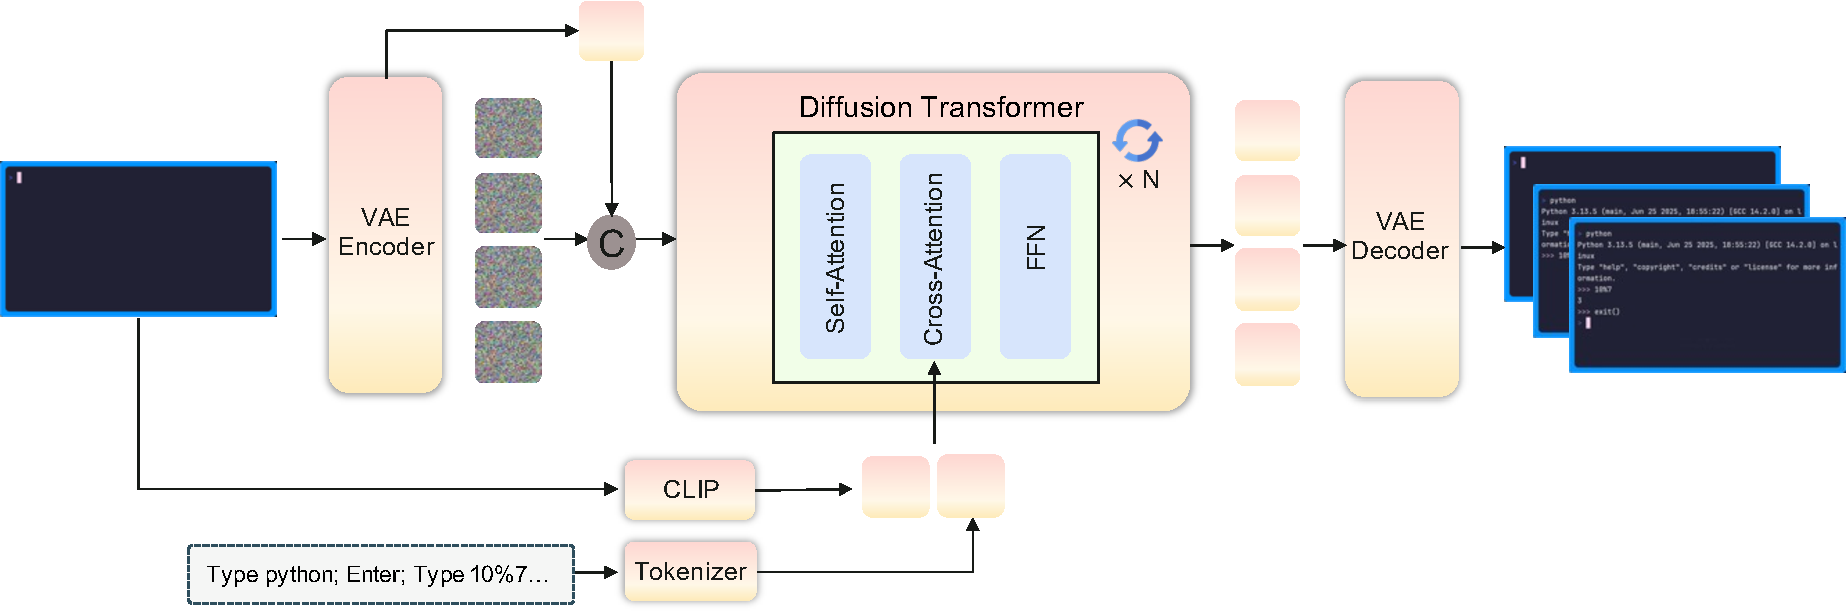
\includegraphics[width=0.8\linewidth]{assets/cligen_7}
  \caption{\cligenGeneralLogo{}\,/\,\cligenCleanLogo{}\,NC$_\text{CLIGen}$ architecture.
  Terminal frames are observations $x_t$.
  A prompt and the first frame seed the conditioning stream.
  The Wan2.1-based latent state $z_t$ rolls forward under the standard I2V sampling scheme.}
  \label{fig:cligen-arch}
\end{figure}






\subsubsection{Implementation Details}

Training uses gradient checkpointing and applies dropout 0.1 to the prompt encoder, CLIP, and VAE modules.
Optimization uses AdamW (learning rate $5\times10^{-5}$, weight decay $10^{-2}$), \texttt{bfloat16} precision, and gradient clipping at 1.0.
%
Training \nccligen{} on CLIGen (General) requires $\sim$15{,}000 H100 GPU hours at batch size 1.
Training on CLIGen (Clean) across both subsets requires $\sim$7{,}000 H100 GPU hours.


\subsubsection{Evaluations}

% Our CLI neural computer achieves high-fidelity rendering and basic interaction.
Unless otherwise noted, NC in this section refers to the current video-based CLI prototype. We report six practical takeaways:
\begin{tcolorbox}[
  colback=metablue!6,
  colframe=metablue!40,
  boxrule=0pt,
  borderline west={1pt}{0pt}{gray!60},
  left=6pt,right=4pt,top=3pt,bottom=3pt]
\small
\begin{itemize}
  \setlength{\itemsep}{3pt}
  \setlength{\topsep}{2pt}
  \item The NC maintains high-fidelity terminal rendering at practical font sizes (e.g., 13\,px), preserving readable interface state.
  \item Prompt specificity is an effective control channel: detailed, literal captions improve text-to-pixel alignment.
  \item On clean but domain-specific data, PSNR/\SSIM~plateau around 25k steps (Figure~\ref{fig:cligen-long-train}), suggesting coverage matters more than longer optimization.
  \item The NC reproduces complex terminal appearances while sustaining multi-step command execution.
  \item Symbolic computation remains the main bottleneck: structured arithmetic reveals reliability limits, motivating stronger symbolic or system-level conditioning.
  \item In our setting, without changing the NC backbone or adding RL, reprompting improves symbolic probes (4\%$\rightarrow$83\%; Figure~\ref{fig:cligen-exp6}), supporting the view that current models are strong renderers but not reasoners (Table~\ref{tab:sora-leads}).
\end{itemize}
\end{tcolorbox}


\exptitle[\cligenGeneralLogo]{1}{The NC stays readable at practical font sizes}


Concurrent work~\citep{rivard2025neuralos} argues that generic natural-image VAEs can perform poorly on structured computer screenshots.
We test this claim directly by applying the Wan2.1 VAE~\citep{wan2025wan} to terminal content.
In our setting, reconstruction quality is primarily governed by font size.
At 13\,px, it is high (40.77\,dB \PSNR, 0.989 \SSIM).
At 6\,px, text exhibits noticeable blurring even when global \PSNR/\SSIM~remain strong, because background regions dominate these metrics.


\begin{figure}[h!]
  \centering
  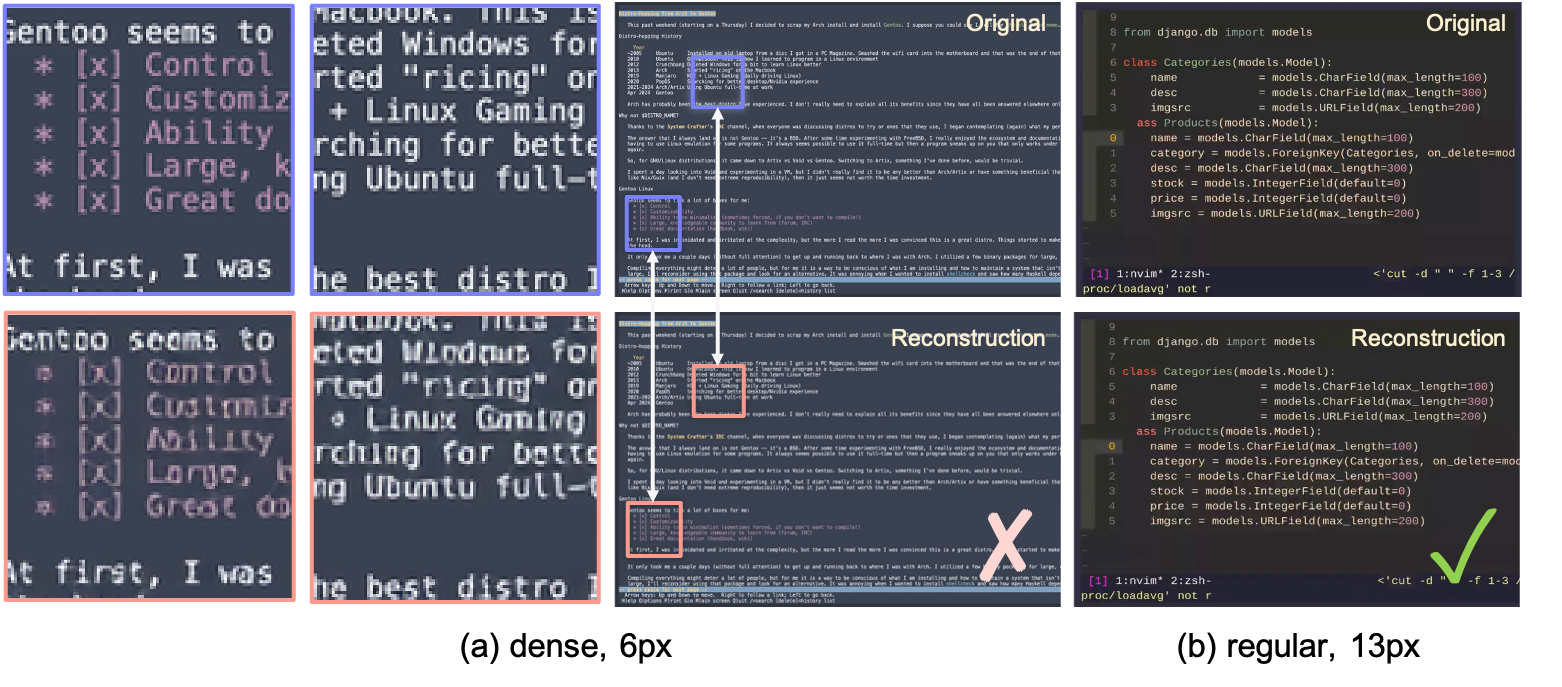
\includegraphics[width=\linewidth]{assets/recon_comp3.png}
    \vspace{-15pt}
\caption{Wan2.1 VAE reconstructions on CLIGen (General) terminal frames at different font sizes.}
  \label{fig:cligen-exp1}

\end{figure}


\begin{wraptable}{r}{0.42\linewidth}
  \vspace{-22pt}
  \captionsetup{type=table,width=\linewidth}
  \centering
  \small
  \rowcolors{2}{metablue!8}{white}
  \caption{Reconstruction quality.}
  \label{tab:cli-vae-recon}
  \setlength{\tabcolsep}{7pt}
  \begin{tabularx}{\linewidth}{l >{\centering\arraybackslash}X}
    \toprule
    \rowcolor{metablue!16} \textbf{Metric} & \textbf{Value} \\
    Average PSNR & 40.77 \\
    Average SSIM & 0.989 \\
    \bottomrule
  \end{tabularx}
  \vspace{-3.9em}
\end{wraptable}
However, a sweep over CLIGen (General) frames shows that this effect is confined to extreme cases (\Cref{fig:cligen-exp1}).
Very small 6\,px fonts and ultra-dense text exhibit localized blurring despite high global \PSNR.
In contrast, the 13\,px terminal font used in CLIGen remains visually sharp across panes and commands. 
These results indicate that the VAE is adequate for regular CLIGen usage and highlight that sensible font choices help ensure stable NC training.

\exptitle[\cligenCleanLogo]{2}{Performance plateaus early and can degrade with prolonged training}

On clean but domain-specific structured interfaces, we find that data quality can matter more than longer training.
In CLIGen (Clean), \PSNR/\SSIM~plateau quickly, suggesting diminishing returns from extended optimization.
After early gains, remaining errors are often driven by artifact-prone supervision (e.g., rendering glitches or rapid screen changes that disrupt temporal alignment).

\begin{wrapfigure}{r}{0.7\linewidth}
  \vspace{-0.8em}
  \centering
  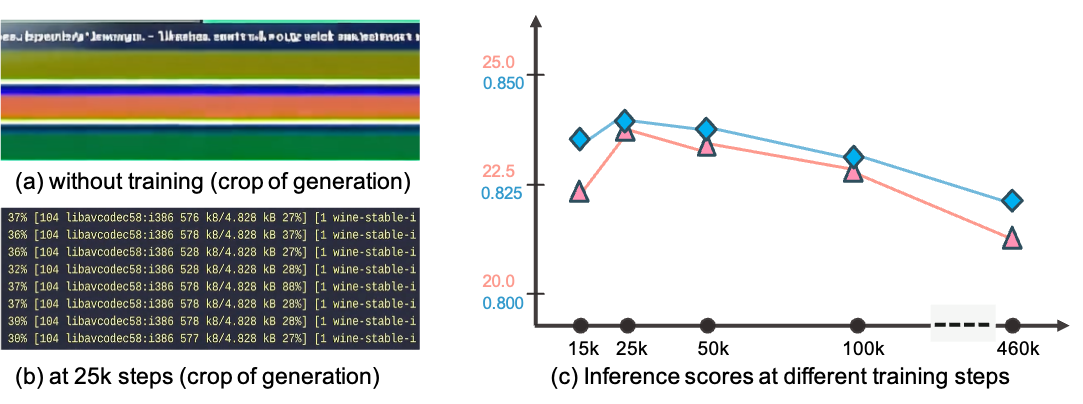
\includegraphics[width=\linewidth]{assets/train_metrics_curve10.png}
  \caption{(a--b) Qualitative generations before and after CLIGen training; (c) CLIGen (Clean) \PSNR/\SSIM~plateau around 25k training steps.}
  \label{fig:cligen-long-train}
  \vspace{-0.8em}
\end{wrapfigure}

Panels (a--b) illustrate the effect of training on CLIGen data.
Without CLIGen fine-tuning, Wan2.1 produces garbled terminal outputs (a).
After 25k steps, the model generates readable text with consistent formatting and color cues (b).

Figure~\ref{fig:cligen-long-train} plots the corresponding \PSNR/\SSIM~curves and indicates a clear efficiency ceiling.
These metrics peak around 25k steps and show little improvement with further training up to 460k steps.
Extended training can even slightly degrade performance.
One plausible explanation is that most learnable structured patterns are acquired early, and further gains require higher-quality, better-paced, or more informative supervision.

\exptitle[\cligenGeneralLogo]{3}{Literal captions drive rendering accuracy}



Caption specificity has a strong effect on terminal rendering quality.
As shown in Table~\ref{tab:cligen-captions}, detailed, literal descriptions improve reconstruction fidelity.
\PSNR increases from 21.90~dB (semantic) to 26.89~dB (detailed), a gain of nearly 5~dB, compared to less specific, high-level semantic descriptions.

The three caption tiers correspond to the same underlying terminal sequence but differ in length and granularity.
\textbf{Semantic} captions (average 55 words) provide high-level summaries (e.g., ``a terminal session generates three cat images'').
\textbf{Regular} captions (average 52 words) include key commands and outputs (e.g., \texttt{ai -i 3 a cute cat}, status messages).
\textbf{Detailed} captions (average 76 words) transcribe screen content more exhaustively, including exact text, colors, and formatting.

\begin{wraptable}{r}{0.42\linewidth}
  \vspace{-1.8em}
  \captionsetup{type=table,width=\linewidth}
  \centering
  \small
  \rowcolors{2}{metablue!8}{white}
  \caption{Caption styles versus TI2V fidelity.}
  \label{tab:cligen-captions}
  \setlength{\tabcolsep}{5pt}
  \begin{tabularx}{\linewidth}{l >{\centering\arraybackslash}X >{\centering\arraybackslash}X >{\centering\arraybackslash}X}
    \toprule
    \rowcolor{metablue!16} \textbf{Prompt style} & \textbf{\PSNR} & \textbf{\SSIM} & \textbf{Avg. words} \\
    Semantic & 21.90 & 0.813 & 55 \\
    Regular & 23.63 & 0.843 & 52 \\
    Detailed & \textbf{26.89} & \textbf{0.867} & \textbf{76} \\
    \bottomrule
  \end{tabularx}
  \vspace{-1.5em}
\end{wraptable}
This progression helps explain why literal descriptions are particularly effective for terminal rendering.
Unlike natural images, which are dominated by global style patterns, terminal frames are governed primarily by text placement.
% Detailed captions act as scaffolding by specifying which tokens appear where, enabling precise text-to-pixel alignment.
% This matches the observed gains as caption specificity increases.
Detailed captions act as scaffolding—explicitly specifying which tokens appear where—thereby enabling precise text-to-pixel alignment.



\exptitle[\cligenCleanLogo]{4}{Neural computers achieve accurate character-level text generation}

\begin{wraptable}{r}{0.42\linewidth}
  \vspace{-0.8em}
  \captionsetup{type=table,width=\linewidth}
  \centering
  \small
  \rowcolors{2}{metablue!8}{white}
  \caption{OCR accuracy versus training.}
  \label{tab:cligen-ocr}
  \setlength{\tabcolsep}{7pt}
  \begin{tabularx}{\linewidth}{l >{\centering\arraybackslash}X >{\centering\arraybackslash}X}
    \toprule
    \rowcolor{metablue!16} \textbf{Steps (k)} & \textbf{Char. acc.} & \textbf{Exact line} \\
    0  & 0.03 & 0.01 \\
    10 & 0.18\,$\color{green!60!black}{\uparrow}_{0.15}$ & 0.05\,$\color{green!60!black}{\uparrow}_{0.04}$ \\
    20 & 0.33\,$\color{green!60!black}{\uparrow}_{0.30}$ & 0.12\,$\color{green!60!black}{\uparrow}_{0.11}$ \\
    30 & 0.41\,$\color{green!60!black}{\uparrow}_{0.38}$ & 0.18\,$\color{green!60!black}{\uparrow}_{0.17}$ \\
    40 & 0.52\,$\color{green!60!black}{\uparrow}_{0.49}$ & 0.26\,$\color{green!60!black}{\uparrow}_{0.25}$ \\
    50 & 0.52\,$\color{green!60!black}{\uparrow}_{0.49}$ & 0.27\,$\color{green!60!black}{\uparrow}_{0.26}$ \\
    60 & \textbf{0.54}\,$\color{green!60!black}{\uparrow}_{0.51}$ & \textbf{0.31}\,$\color{green!60!black}{\uparrow}_{0.30}$ \\
    \bottomrule
  \end{tabularx}
  \vspace{-0.8em}
\end{wraptable}

Beyond PSNR and SSIM, character-level accuracy is a more direct metric for terminal rendering.
Character-level accuracy requires explicit pixel-to-text correspondence.
For CLIGen (Clean), we apply Tesseract to five uniformly sampled (ground-truth, generated) frame pairs per video and normalize whitespace.
We then compute two metrics (full protocol in Appendix~\ref{appendix:pipeline}).
Character accuracy uses the Levenshtein distance between concatenated ground-truth and generated texts.
Exact-line accuracy measures the fraction of ground-truth lines whose normalized content exactly matches the prediction at the same line index.

Table~\ref{tab:cligen-ocr} shows that our models achieve substantial text rendering accuracy under this protocol.
Character accuracy increases from 0.03 at initialization to 0.54 at 60k steps, with exact-line matches reaching 0.31 (0.26 by 40k).
Most gains occur within the first 40k steps, followed by smaller refinements thereafter.
These OCR-based metrics capture properties beyond perceptual similarity. 
Accurately generating terminal characters requires modeling text structure, font rendering, and spatial relationships.
These are core competencies for interactive neural computer systems.
This level of character-level precision is a step toward usable, not just plausible, terminal interfaces.



\exptitle[\cligenCleanLogo]{5}{Does this NC instantiation show native CLI reasoning?}

\providecommand{\wanicon}{\raisebox{-0.25ex}{
\includegraphics[height=1.00em]{assets/wan_icon.png}}}
\providecommand{\veoicon}{\raisebox{-0.25ex}{
\includegraphics[height=1.00em]{assets/veo_ICON.png}}}
\providecommand{\soraicon}{\raisebox{-0.25ex}{
\includegraphics[height=1.00em]{assets/sora_icon.png}}}
\begin{wraptable}{r}{0.50\linewidth}
  \vspace{-1.0em}
  \captionsetup{type=table,width=\linewidth}
  \centering
  \small
  \rowcolors{2}{metablue!8}{white}
  \caption{Arithmetic probe accuracy (100 problems sampled from a 1{,}000-problem held-out pool).}
  \label{tab:cligen-arith}
  \setlength{\tabcolsep}{8pt}
  \begin{tabularx}{\linewidth}{l >{\centering\arraybackslash}X}
    \toprule
    \rowcolor{metablue!16} \textbf{Model} & \textbf{Accuracy} \\
    \wanicon\;Wan2.1 & 0\% \\
    \cligenCleanLogo{}\;\nccligen{} & 4\% \\
    \veoicon\;Veo3.1 & 2\% \\
    \soraicon\;Sora2 & \textbf{71}\% \\
    % \cligenCleanLogo{}\;\nccligen{} + reprompt & \textbf{83\%} \\
    \bottomrule
  \end{tabularx}
   \vspace{-1.0em}
\end{wraptable}
We also probe symbolic computation with CLI arithmetic tasks.
These tasks are a sharp stress test for symbolic reliability: humans answer them instantly, yet current NC instantiations often fail on seemingly simple symbolic operations.

Our arithmetic probe presents basic mathematical operations through terminal interactions.
We reserve a held-out pool of 1{,}000 math problems and randomly sample 100 problems as the final evaluation set.
Table~\ref{tab:cligen-arith} shows that current video models, including this NC instantiation, struggle on these symbolic tasks.
Wan2.1 achieves 0\% accuracy, our \nccligen{} model reaches 4\%, and Veo3.1 manages 2\%—all far below human-level performance on these fundamental tasks.
%
These results contrast with common claims of strong symbolic reasoning in current video models.
Sora2's 71\% accuracy is a notable outlier and may reflect system-level advantages or additional training beyond our current setup.
Overall, native symbolic reasoning remains an open challenge for current video-based NC~instantiations.




The poor arithmetic-probe performance in Table~\ref{tab:cligen-arith} raises a key question.
Does this prototype require specialized reinforcement learning to achieve reliable symbolic computation, or can stronger conditioning substantially narrow this gap?
% Sora2's 71\% accuracy suggests several possible explanations, which we examine systematically in Table~\ref{tab:sora-leads}. 


\exptitle[\cligenCleanLogo]{6}{Does this NC instantiation require RL for symbolic probes?}
\begin{wrapfigure}{r}{0.49\linewidth}
  \vspace{-1.8em}
  \centering
  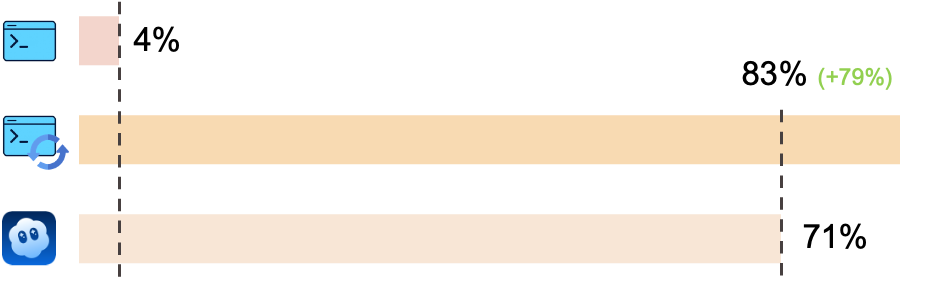
\includegraphics[width=\linewidth]{assets/cligen_exp6v3.png}
  \caption{Reprompting boosts performance to 83\%.}
  \label{fig:cligen-exp6}
  \vspace{-1.0em}
\end{wrapfigure}

As shown in Figure~\ref{fig:cligen-exp6}, \nccligen{} accuracy on CLIGen (Clean) arithmetic tasks rises from 4\% to 83\% under reprompting.
This suggests that system-level conditioning can be an effective first lever for improving performance on symbolic probes.
It is complementary to (rather than strictly requiring) RL-based training pipelines.
%
More generally, the success of reprompting highlights how sensitive symbolic-probe outcomes are to the conditioning interface.
Much of the apparent ``reasoning'' gain can come from better specification and instruction-following rather than new native computation.
For the arithmetic subset, we include the correct answer explicitly in roughly half of the training captions to encourage reliable rendering of the output string.
Because reprompting can similarly provide stronger hints (or even outsource computation to an external text system), we interpret the gain primarily as evidence of steerability.
It also shows faithful rendering of conditioned symbolic content.
We do not treat it as a clean demonstration that the NC backbone performs arithmetic internally.




\begin{table}[h]
  \captionsetup{type=table,width=\linewidth}
  \centering
  \small
  \rowcolors{2}{metablue!8}{white}
\caption{Hypotheses for Sora2's advantage.}
 \vspace{-4pt}
  \label{tab:sora-leads}
  \setlength{\tabcolsep}{6pt}
  \begin{tabularx}{\linewidth}{l X}
    \toprule
    \rowcolor{metablue!16} \textbf{Factor} & \textbf{Implication} \\
    \tikz[baseline=-0.35ex]{\node[fill=metablue, text=white, circle, inner sep=1.2pt, font=\scriptsize\bfseries] {1};} Stronger base + similar data & Higher intrinsic arithmetic; symbolic capability may be baked in \\
    \tikz[baseline=-0.35ex]{\node[fill=orange!85!red, text=white, circle, inner sep=1.2pt, font=\scriptsize\bfseries] {2};} Additional RL training & Reward shaping teaches math beyond diffusion; could transfer to CLI \\
    \tikz[baseline=-0.35ex]{\node[fill=teal!70!black, text=white, circle, inner sep=1.2pt, font=\scriptsize\bfseries] {3};} System-level reprompt/recaption & LLM computes answers; strong conditioning drives generation \\
    \bottomrule
  \end{tabularx}
\end{table}

The evidence supports system-level conditioning as a practical path forward for this NC instantiation.
Among the three hypotheses for improving arithmetic-probe performance—stronger base models, reinforcement learning, or enhanced conditioning—our results most strongly favor the third approach.
The gain from reprompting (4\%$\rightarrow$83\%), achieved without modifying the underlying NC backbone, is substantial.
It shows that measured ``reasoning'' on these probes is highly sensitive to specification and conditioning.
We therefore do not treat it as direct evidence of native arithmetic inside the NC backbone.

In our setting, strategic conditioning yields larger symbolic-probe gains than the RL pipeline we tested.
Evaluations should therefore distinguish native computation from conditioning-assisted performance when assessing reasoning capabilities in current video-based NC instantiations.






\subsubsection{Visualizations}

\noindent\textbf{(1) \cligenGeneralData{} visualizations.}
Qualitative samples highlight the breadth of real-world terminal dynamics captured in CLIGen (General): ANSI escape sequences that repaint regions with changing foreground/background colors, incremental command entry with syntax highlighting and cursor edits, classic shell prompts and system outputs, long-running jobs with rapidly scrolling and color-coded package logs, full-screen TUIs such as partition editors, and progress dashboards with updating bars, counts, and ETAs.
These traces emphasize that ``looking correct'' requires maintaining terminal geometry, palette transitions, and cursor state frame-by-frame.

\noindent\textbf{(2) \cligenCleanData{} REPL visualizations.}
In contrast to open-world traces, CLIGen (Clean) REPL samples are scripted and temporally well-paced (Figures~\ref{fig:cligen-clean-viz-a}--\ref{fig:cligen-clean-viz-d}; additional examples are in Appendix~\ref{appendix:cligen-samples}).
Each sample includes an explicit action trace (e.g., \texttt{Sleep}, \texttt{Type}, \texttt{Enter}, arrow keys, \texttt{Hide}) alongside rendered terminal frames, making the action-to-pixel link visually unambiguous.
The key insight is that these scripted traces isolate rendering-and-control errors from semantic ambiguity: with explicit actions, failures are dominated by low-level mechanics (cursor placement, character edits, monospace alignment, line breaks, temporal consistency).

\noindent\textbf{(3) \cligenCleanData{} math visualizations.}
Figures~\ref{fig:cligen-clean-math-comp-a}--\ref{fig:cligen-clean-math-comp-c} compare math REPL rollouts, and Figures~\ref{fig:cligen-clean-math-rep-a}--\ref{fig:cligen-clean-math-rep-c} show reprompting cases.
Together they highlight why arithmetic probes should separate native computation from answer-conditioned rendering.
All full-resolution pages are in Appendix~\ref{appendix:vis}; below we keep clickable thumbnails at the original location for quick navigation.

\newcommand{\CliThumbPageHeader}[1]{%
  \par\noindent\makebox[\linewidth][c]{%
    \fcolorbox{metablue!45}{metablue!5}{%
      \begin{minipage}{0.94\linewidth}
        \centering
        \vspace{0.22em}
        {\large\bfseries #1}\par
        \vspace{0.1em}
        {\scriptsize\textsf{\color{metablue!85!black}Click any thumbnail to jump to its full-resolution page in Appendix}}\par
        \vspace{0.18em}
      \end{minipage}
    }%
  }\par\vspace{0.58em}%
}
\newcommand{\CliThumbPageHeaderSimple}[1]{%
  \par\noindent\makebox[\linewidth][c]{%
    \fcolorbox{metablue!45}{metablue!5}{%
      \begin{minipage}{0.94\linewidth}
        \centering
        \vspace{0.22em}
        {\large\bfseries #1}\par
        \vspace{0.16em}
      \end{minipage}
    }%
  }\par\vspace{0.58em}%
}
\newcommand{\CliThumbPageHeaderPlain}[1]{%
  {\par\noindent\centering\Large\bfseries #1\par}
  {\par\noindent\centering%
    \begin{tcolorbox}[
      enhanced,
      boxrule=0.85pt,
      colframe=orange!80!black,
      colback=yellow!14,
      arc=5.5pt,
      left=6pt,right=6pt,top=2.5pt,bottom=2.5pt,
      width=0.78\linewidth
    ]
      \centering\small\bfseries\sffamily\color{orange!85!black}
      Click any thumbnail to jump to its full-resolution page in Appendix
    \end{tcolorbox}\par
  }
  \vspace{0.26em}%
}
\newcommand{\CliThumbPageFrame}{%
  \begin{tikzpicture}[remember picture,overlay]
    \draw[
      draw=black,
      line width=1.9pt,
      rounded corners=14pt
    ]
      ([xshift=0.48cm,yshift=-0.48cm]current page.north west)
      rectangle
      ([xshift=-0.48cm,yshift=0.48cm]current page.south east);
  \end{tikzpicture}%
}
\newcommand{\CliThumbCard}[4]{%
  \par\noindent\makebox[\linewidth][c]{%
    \hyperref[#1]{%
      \begin{tikzpicture}
        \node[inner sep=0pt] (img) {\includegraphics[width=#4\linewidth,keepaspectratio]{#2}};
        \node[
          anchor=south east,
          xshift=-0.38em,
          yshift=0.26em,
          fill=white,
          fill opacity=0.93,
          text opacity=1,
          draw=metablue!50,
          rounded corners=1.5pt,
          inner xsep=0.45em,
          inner ysep=0.2em,
          minimum width=8.4em,
          align=center,
          font=\scriptsize\bfseries,
          text=metablue!90!black
        ] at (img.south east) {#3};
      \end{tikzpicture}%
    }%
  }\par\vspace{0.28em}%
}
\newcommand{\CliThumb}[4]{\CliThumbCard{#1}{#2}{#3}{#4}}

\clearpage
\newgeometry{top=0.9cm,bottom=1.35cm,left=0.9cm,right=0.9cm,includefoot,footskip=18pt}
\thispagestyle{plain}
\hypertarget{main-cligen-vis-thumbs}{}
\hypertarget{main-cligen-vis-thumbs-p1}{}
\hypertarget{main-cligen-vis-thumbs-p2}{}
\CliThumbPageFrame
\CliThumbPageHeaderPlain{CLIGen Visualization Thumbnails}
\noindent\begin{tabular}{@{}p{0.495\linewidth}!{\color{metablue!55}\vrule width 0.8pt}p{0.495\linewidth}@{}}
\begin{minipage}[t]{\linewidth}
  \vspace*{0pt}
  \centering
  {\small\bfseries \cligenGeneralLogo{}\ CLIGen (General) Visualizations}\par
  \vspace{0.14em}
  \CliThumb{fig:cligen-general-viz-1}{assets/cligen_general_1.pdf}{\cligenGeneralLogo{}\ Samples A}{0.72}
  \CliThumb{fig:cligen-general-viz-2}{assets/cligen_general_2.pdf}{\cligenGeneralLogo{}\ Samples B}{0.72}
  \CliThumb{fig:cligen-general-viz-3}{assets/cligen_general_3.pdf}{\cligenGeneralLogo{}\ Samples C}{0.72}
\end{minipage}
&
\begin{minipage}[t]{\linewidth}
  \vspace*{0pt}
  \centering
  {\small\bfseries \cligenCleanLogo{}\ CLIGen (Clean) Visualizations}\par
  \vspace{0.14em}
  \CliThumb{fig:cligen-clean-viz-a}{assets/cligen_clean_1.pdf}{\cligenCleanLogo{}\ Samples A}{0.97}
  \CliThumb{fig:cligen-clean-viz-b}{assets/cligen_clean_2.pdf}{\cligenCleanLogo{}\ Samples B}{0.97}
  \CliThumb{fig:cligen-clean-viz-c}{assets/cligen_clean_3.pdf}{\cligenCleanLogo{}\ Samples C}{0.97}
  \CliThumb{fig:cligen-clean-viz-d}{assets/cligen_clean_4.pdf}{\cligenCleanLogo{}\ Samples D}{0.97}
\end{minipage}
\end{tabular}
\restoregeometry
\par\justifying

\clearpage
\newgeometry{top=0.9cm,bottom=1.35cm,left=0.9cm,right=0.9cm,includefoot,footskip=18pt}
\thispagestyle{plain}
\hypertarget{main-cligen-vis-thumbs-p3}{}
\hypertarget{main-cligen-vis-thumbs-p4}{}
\CliThumbPageFrame
\CliThumbPageHeaderPlain{CLIGen Visualization Thumbnails}
\noindent\begin{tabular}{@{}p{0.495\linewidth}!{\color{metablue!55}\vrule width 0.8pt}p{0.495\linewidth}@{}}
\begin{minipage}[t]{\linewidth}
  \vspace*{0pt}
  \centering
  {\small\bfseries \cligenCleanLogo{}\ CLIGen (Clean) Math Comparison}\par
  \vspace{0.14em}
  \CliThumb{fig:cligen-clean-math-comp-a}{assets/cligen_math_comp1.pdf}{\cligenCleanLogo{}\ Samples A}{0.76}
  \CliThumb{fig:cligen-clean-math-comp-b}{assets/cligen_math_comp2.pdf}{\cligenCleanLogo{}\ Samples B}{0.76}
  \CliThumb{fig:cligen-clean-math-comp-c}{assets/cligen_math_comp3.pdf}{\cligenCleanLogo{}\ Samples C}{0.76}
\end{minipage}
&
\begin{minipage}[t]{\linewidth}
  \vspace*{0pt}
  \centering
  {\small\bfseries \cligenCleanLogo{}\ CLIGen (Clean) Math Reprompting}\par
  \vspace{0.14em}
  \CliThumb{fig:cligen-clean-math-rep-a}{assets/cligen_math_rep1.pdf}{\cligenCleanLogo{}\ Samples A}{0.98}
  \CliThumb{fig:cligen-clean-math-rep-b}{assets/cligen_math_rep2.pdf}{\cligenCleanLogo{}\ Samples B}{0.98}
  \CliThumb{fig:cligen-clean-math-rep-c}{assets/cligen_math_rep3.pdf}{\cligenCleanLogo{}\ Samples C}{0.98}
\end{minipage}
\end{tabular}
\restoregeometry
\par\justifying
